\subsubsection{Theory Overview}
\label{subseq:iterative-theory}


% the first choice
Given an initial guess, iterative methods generate a sequence of successively improving approximated solutions. The methods are preferred for their relatively low computational cost per iteration and storage requirements $O(nnz)$. In essence, the methods make use of simple linear algebra kernels  at each iteration and thus can handle matrix sparsity efficiently.\\



The family of iterative methods consists of two distinct classes, namely: stationary and Krylov methods. Nowadays, Krylov methods dominate in the filed of scientific computing because of it is rather fast convergence in case of solving of well conditioned systems.\\


The most well-known methods among the Krylov family are Conjugate Gradient (CG) in case of symmetric positive definite matrices, Minimal Residual Method (MINRES) for symmetric indefinite systems and Generalized Minimal Residual Method (\gls{gmres}) for non-symmetric systems of linear equations. There also exist different variants of \gls{gmres} such as Biconjugate Gradient Method (BiCG), Biconjugate Gradient Stabilized Method (BiCGSTAB), etc.\\


The key idea is a construction of an approximate solution of a system of linear equations as a linear combination of vectors $b$, $Ab, \:\: A^2b, \:\: A^3b, \dots A^{n}b$. The combination defines a subspace, also known as Krylov subspace $\mathcal{K}_{n}$. At each iteration, the subspace is expanded by adding and evaluating the next vector in the sequence. Essentially, the methods convert solution of a system of a linear equations to a minimization problem and search for a solution in the corresponding subspace.\\


For example, \gls{gmres} aims to minimize the Euclidean norm of the residual $r_{m}$ of a solution vector $x_{m}$ in $m$th Krylov subspace $\mathcal{K}_{m}$. However, the basis vectors of Krylov subspace $\mathcal{K}_{m}$ are usually close to linearly dependent and, thus, solution vector $x_{m}$ is constructed in an orthonormal basis $U_{m}$ which forms the same subspace $\mathcal{K}_{m}$.\\


\begin{equation} \label{eq:Gmres-1}
	r_{m} = \underset{x \in U_m}{min}||Ax_{m} - b||^2 =  \underset{x \in U_m}{min}||AU_m y_{m} - b||^2
\end{equation}

where the vector $x$ can be written in the basis $U_m$ as:

\begin{equation} \label{eq:Gmres-2}
		x = U_{m} y
\end{equation}

In the general case, orthogonalization of the basis can be performed in different ways. Saad and Schultz, in work \cite{sparse-la:gmrese-origin}, proposed to use the Arnoldi process for constructing an $l_2$-orthogonal basis. As a result, equation \ref{eq:Gmres-1} can be written in a form:  \\

\begin{equation} \label{eq:Gmres-3}
	r_{m} = \underset{x \in U_m}{min}||U_{m+1}H_{m+1,m} y_{m} - ||b||u_1||^2 = \\
	\underset{x \in U_m}{min}||H_{m+1,m} y_{m} - ||b||e_1||^2 
\end{equation}

where $H_{m}$ is an upper Hessenberg matrix i.e. the matrix with zeros below the first sub-diagonal. Application of the Givens rotation algorithm results in computing of the corresponding $QR$ decomposition of Hessenberg matrix $H_{m}$. After the substitution of matrix $H_{m}$ with the decomposition and some mathematical transformations, equation \ref{eq:Gmres-3} can be written as follows:\\

 
\begin{equation} \label{eq:Gmres-4}
	r_{m} = \\
	\underset{x \in U_m}{min}||Q^{T}Ry_{m} - ||b||e_{1}||^2 = \\
	\underset{x \in U_m}{min}||\Big(\begin{array}{c c}R_m \\ 0 \\\end{array}\Big) y_{m} - \Big(\begin{array}{c c} \tilde{b_m} \\ \tilde{b_{n-m}} \\\end{array}\Big)||^2
\end{equation}

Now, the minimization problem \ref{eq:Gmres-4} can be solved as:\\

\begin{equation} \label{eq:Gmres-5}
	R_m y_{m} = \tilde{b_m}
\end{equation}

Given the decomposition of a vector in orthonormal basis $U_{m}$, equation\ref{eq:Gmres-2}, solution vector $x_{m}$ can be written as:\\

\begin{equation} \label{eq:Gmres-6}
	x_m = U_m y_{m}  
\end{equation}


The solution significantly improves with growth of subspace $\mathcal{K}_{m}$. This, in turn, leads to a considerable increase of computational cost and storage space, as a result. Therefore, the algorithm usually runs till 20 - 50 column vector evaluations of the Krylov subspace and restarts using the computed approximate solution as an initial guess for the next iteration.\\


\subsubsection{Parallelization Aspects}
\label{subseq:iterative-parallel-aspects}


% data parallelism
In the general case, iterative methods usually make use of dot and matrix-vector products for solving systems of linear equations. Application of these linear algebra kernels allows to efficiently handle sparsity of linear systems and thus reduce computational complexity of the methods. Additionally, it allows to distribute vectors and matrices across multiple compute-units and solve systems of equations in parallel efficiently exploiting data parallelism. Hence, the main drop of parallel performance mainly comes from process-communication overheads.\\


However, some methods can have sequential parts that may effect on parallel performance as well. For instance, a triangular solve operation,  equation \ref{eq:Gmres-5}, of the \gls{gmres} method is usually computed in a single processor because of its small size which depends on the number of iterations before the restart. Hence, if the underlying system of equations is relatively small then such sequential operations can become a bottleneck in solving the corresponding system.\\


%In such cases, these operations can become a bottleneck if the underlying system of equations is relatively small as well. \\



%\todo{figure bla shows different restarts}
%Figure \ref{fig:gmres-strong-scaling-speed-up} shows strong scaling performance results of the default \gls{gmres} solver from the \gls{petsc} library. The solver was set up without any preconditioner and 50 iterations as the restart. Additionally no stop criteria was specified except the maximum number iterations which was equal to 100. The \textit{spread} process pinning strategy, described in section \ref{subseq:matrix-sets-and-hardware}, was used. It is well-known that all iterative methods are memory bound due to indirect memory addressing caused by sparse matrix storage schemes. Hence equal process distribution can help reduce the load on memory channels since it is an obvious bottleneck for this type of applications. \\


%Four matrices were chosen form the \gls{grs} matrix set for the tests, namely: cube-64, cube-645, k3-2 and k3-18. The information about the matrices is summarized in table \ref{table:grs-matrix-set}. As we expected, we can observe strong deviation of our results from the ideal speed-up line when the number of processes exceeds 10.\\


%\figpointer{\ref{fig:gmres-strong-scaling-speed-up}}

%It should be mentioned that parallelization overheads, introduced by such \gls{mpi} operations as \gls{mpi}\_Send, \gls{mpi}\_Recv, \gls{mpi}\_Allreduce, etc., also have their impact on performance of the algorithm.\\



%\figpointer{\ref{fig:gmres-strong-scaling-speed-up}}
%\begin{figure}[htpb]
%  \centering
%  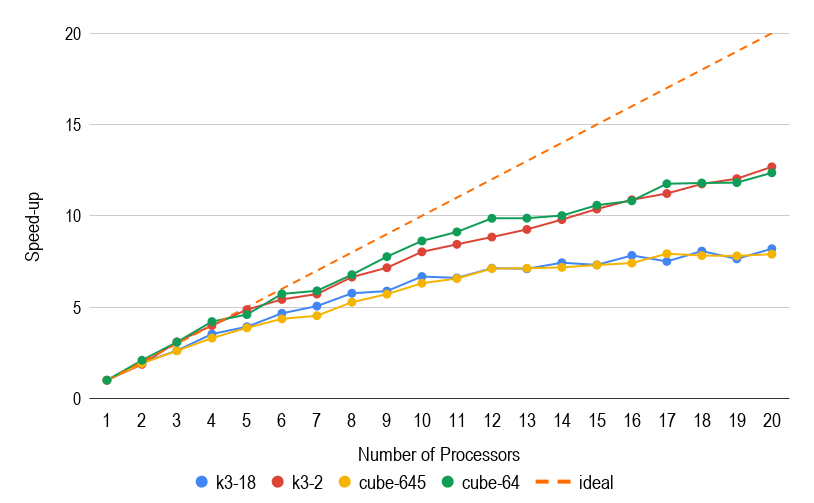
\includegraphics[width=0.7\textwidth]{figures/%chapter-2/gmres-strong-scaling-speedup.png}
%\caption{\gls{gmres} strong scaling speed-up}
%\label{fig:gmres-strong-scaling-speed-up}
%\end{figure}



\subsubsection{Preconditioners}
\label{subseq:iterative-preconditioners}
% start discussion about preconditioning
The most important criteria of Krylov methods is convergence. The convergence of iterative methods strongly depends on a matrix and, in particular, on its condition number. For instance, equation \ref{eq:Gmres-7} shows dependence of an error reduction in the solution on the corresponding matrix condition number in case of CG method. It can be clearly observed that a big condition number results in a very slow error reduction and, therefore, in a slow convergence rate.\\

\begin{equation} \label{eq:Gmres-7}
	|| e^i ||_A \leq 2 ( \frac{\sqrt k - 1}{\sqrt k + 1} )^i || e^0 ||_A
\end{equation}

where $k = \frac{\lambda_{max}}{\lambda_{min}}$ - a matrix condition number\\

%1. In practice, a system of equation is preconditioned with a matrix $P$ which allows to lower the condition number of the modified matrix.\\

In practice, a linear transformation, known as preconditioning, is applied to the original system in order to reduce its condition number. As a result, the solution process of the modified system is significantly accelerated. The transformation can be applied in different ways. For instance, equations \ref{eq:pcn-1} and \ref{eq:pcn-2} show applications of a preconditioning matrix $P$ from left and right sides, respectively.\\


\begin{equation} \label{eq:pcn-1}
	PAx = Pb
\end{equation}


\begin{equation} \label{eq:pcn-2}
	AP(P^{-1}x) = b
\end{equation}


In the general case, a good preconditioning algorithm has to result in \textit{low computational cost, low storage space and a low condition number of the transformed system}. Additionally, computations of large linear systems require an algorithm to be adapted for parallel execution as well.\\


There exist numerous techniques to compute a preconditioner $P$ for a given a matrix $A$ e.g. (point) Jacobi, Block-Jacobi, incomplete $LU$ decomposition (ILU), multilevel ILU (ILU(p)), threshold ILU (ILUT), incomplete Cholesky factorization (IC), sparse approximate inverse (SPAI), multigrid as a preconditioner, etc. Practice has been shown that some techniques can work particularly well for matrices derived from a certain \gls{pde} or a system of \gls{pde}s e.g. Poisson, Navier\-Stokes, etc., and discretized in a certain way. However, \textit{sometimes it can take a quite considerable amount of time to tune a particular preconditioning algorithm in order fulfill all above listed requirements}.\\


As it can be clearly observed from table \ref{table:grs-matrix-set}, all matrices contained in \gls{grs} matrix set are very ill-conditioned and, as a result, require suitable linear transformations. \gls{petsc} provides various preconditioning methods as well as access to some external preconditioning libraries. Table \ref{table:preconditioners} contains some widely-used preconditioning algorithms available in \gls{petsc} capable to run in parallel on distributed-memory machines as well as their short descriptions and tuning parameters.\\


\begin{table}[h!]
\small
\centering
\begin{tabular}{|c|c|c|c|c|}
\hline
\begin{tabular}[c]{@{}c@{}}Package\\ name\end{tabular}     & Origin                                                   & Method                                                        & \begin{tabular}[c]{@{}c@{}}Tuning\\ parameters\end{tabular}                                                                                                                            & Comments                                                                  \\ \hline
block Jacobi                                               & PETSc                                                    & block Jacobi                                                  & \begin{tabular}[c]{@{}c@{}}-pc\_bjacobi\_blocks\\ -sub\_pc\_type\end{tabular}                                                                                                          & -                                                                         \\ \hline
\begin{tabular}[c]{@{}c@{}}additive\\ Schwarz\end{tabular} & PETSc                                                    & \begin{tabular}[c]{@{}c@{}}additive\\ Schwarz\end{tabular}    & \begin{tabular}[c]{@{}c@{}}-pc\_asm\_blocks\\ -pc\_asm\_overlap\\ -pc\_asm\_type\\ -pc\_asm\_local\_type\\ -sub\_pc\_type\end{tabular}                                                 & -                                                                         \\ \hline
euclid                                                     & hypre                                                    & ILU(k)                                                        & \begin{tabular}[c]{@{}c@{}}-nlevel\\ -thresh\\ -filter\end{tabular}                                                                                                                    & \begin{tabular}[c]{@{}c@{}}deprecated\\ form\\ PETSc\end{tabular}         \\ \hline
pilut                                                      & hypre                                                    & ILU(t)                                                        & \begin{tabular}[c]{@{}c@{}}-pc\_hypre\_pilut\_tol\\ -pc\_hypre\_pilut\_maxiter\\ -pc\_hypre\_pilut\_factorrowsize\end{tabular}                                                         & -                                                                         \\ \hline
parasail                                                   & hypre                                                    & SPAI                                                          & \begin{tabular}[c]{@{}c@{}}-pc\_hypre\_parasails\_nlevels\\ -pc\_hypre\_parasails\_thresh\\ -pc\_hypre\_parasails\_filter\end{tabular}                                                 & -                                                                         \\ \hline
SPAI                                                       & \begin{tabular}[c]{@{}c@{}}Grote,\\ Barnard\end{tabular} & SPAI                                                          & \begin{tabular}[c]{@{}c@{}}-pc\_spai\_epsilon\\ -pc\_spai\_nbstep\\ -pc\_spai\_max\\ -pc\_spai\_max\_new\\ -pc\_spai\_block\_size\\ -pc\_spai\_cache\_size\end{tabular}                & -                                                                         \\ \hline
BoomerAMG                                                  & hypre                                                    & \begin{tabular}[c]{@{}c@{}}algebraic\\ multigrid\end{tabular} & \begin{tabular}[c]{@{}c@{}}-pc\_hypre\_boomeramg\_cycle\_type\\ -pc\_hypre\_boomeramg\_max\_levels\\ -pc\_hypre\_boomeramg\_max\_iter\\ -pc\_hypre\_boomeramg\_tol\\ etc.\end{tabular} & \begin{tabular}[c]{@{}c@{}}39 tuning\\ parameters\\ in total\end{tabular} \\ \hline
\end{tabular}
\caption{A list of parallel preconditioning algorithms available in \gls{petsc}}
\label{table:preconditioners}
\end{table}

Detailed descriptions of all tuning parameters listed in table \ref{table:preconditioners} can be found in either \gls{petsc} or Hypre user’s manuals, \cite{balay2018petsc} and \cite{falgout2010hypre}, respectively.\\


It is worth mentioning both block Jacobi and additive Schwarz algorithms 
split the original system into smaller blocks where each block is usually computed on a single processor. Therefore, these algorithms require an explicit specification of another preconditioning algorithm  or a linear solver, called as sub-preconditioner, for local block computations. As an example, code listing \ref{lst:petsc-preconditioner-setups} shows usage of a \textit{sequential} \gls{petsc} built-in $LU$ matrix decomposition subroutine as a sub-preconditioner for the block Jacobi algorithm. As a result, the number of tuning parameters for these two algorithms can grow significantly.\\


\begin{lstlisting}[language=python, caption={An example of usage of a PETSc built-in sparse direct linear solver as a sub-preconditioner for a PETSc Block Jacobi preconditioning algorithm}, frame=single, label={lst:petsc-preconditioner-setups}]
-pc_bjacobi_blocks 4
-sub_pc_type lu
-pc_factor_mat_ordering_type rcm
-pc_factor_pivot_in_blocks true
\end{lstlisting}
